\chapter{Numerical Characterization of Shear Wave Speed Quantification}
	\label{chap:shear}
	\section{Introduction}
		Shear wave speed quantification offers the most desirable method of detecting early deep tissues injuries as it takes the transducer-generated external deformation force that is the chief benefit of ARFI imaging and combines it with a quantitative measure of tissue elasticity rather than the qualitative measures used in both quasi-static elastography and ARFI imaging. Specifically, monitoring the speed of shear waves that are generated in the tissue as a response to a localized acoustic radiation force allows the calculation of tissue stiffness which may again be used as an analogue of tissue health. Further, since the technique is quantitative in nature, tissue stiffness may be accurately tracked over time, enabling physicians to appropriately monitor the progression and treatment of a given deep tissue injury on a per-patient basis.

	\section{Method}
		In order to investigate the sensitivity and applicability of shear wave speed quantification for the early detection of deep tissue injuries, a combination of k-space pseudospectral models of acoustic wave propagation and time-domain finite-element models of tissue deformation were employed. The theory and procedure behind both the generalized acoustic simulations using k-space pseudospectral models and time-dependent solid mechanics finite-element models used here were presented in Chapter \ref{chap:arfi}. As an alternative to monitoring the dynamic response of tissue at the focal point as in ARFI imaging, shear wave speed quantification tracks the velocity of shear waves which radiate laterally outward from the focal point of an ARFI load. If the focal point is positioned such that the generated shear waves propagate through a lesionous region and the speed of the generated shear wave is monitored, the stiffness of that region may be calculated.

		\subsection{Shear Wave Speed}
			The foundation of shear wave speed quantification with regards to detecting lesionous regions lies in the quantifiable relationship between shear wave speeds and tissue stiffness. This relationship between shear wave speed and tissue stiffness is derived here, assuming a linear elastic, isotropic material. Soft tissue is generally considered a viscoelastic material and as such modifications to the linear elastic wave speed are taken into account.

			Equation \ref{equ:shear_constitutive} represents the constitutive equation of a linear elastic material where the strain tensor is defined as per equation \ref{equ:shear_strain_tensor} such that equation \ref{equ:shear_constitutive_complete} holds true.

			\begin{equation}
				\label{equ:shear_constitutive}
				\sigma_{ij} = \lambda \delta_{ij} \varepsilon_{kk} + 2 \mu \varepsilon_{ij}
			\end{equation}

			\begin{equation}
				\label{equ:shear_strain_tensor}
				\varepsilon_{ij} = \frac{1}{2}\left(u_{i,j} + u_{j,i}\right)
			\end{equation}

			\begin{equation}
				\label{equ:shear_constitutive_complete}
				\sigma_{ij} = \lambda \varepsilon_{ii} \delta_{ij} + \mu \left(u_{i,j} + u_{j,i}\right)
			\end{equation}

			Neglecting time-invariant body loads, the balance of linear momentum is given for a linear elastic continuum is given in equation \ref{equ:shear_balance_momentum}.

			\begin{equation}
				\label{equ:shear_balance_momentum}
				\sigma_{ij,j} = \rho \ddot{u_i}
			\end{equation}

			Substituting equation \ref{equ:shear_constitutive_complete} into equation \ref{equ:shear_balance_momentum} yields equation \ref{equ:shear_momentum_constitutive} which may be rearranged into equation \ref{equ:shear_momentum_constitutive_rearranged} by noting that $\varepsilon_{ii,j} = u_{j,ij}$.

			\begin{equation}
				\label{equ:shear_momentum_constitutive}
				\lambda \varepsilon_{ii,j} + \mu\left(u_{i,jj} + u_{j,ij}\right) = \rho \ddot{u_i}
			\end{equation}

			\begin{equation}
				\label{equ:shear_momentum_constitutive_rearranged}
				\rho \ddot{u_i} = \left(\lambda + \mu\right)u_{j,ji} + \mu u_{i,jj}
			\end{equation}

			Utilizing the Helmholtz decomposition of the particle displacement given in equation \ref{equ:shear_helmholtz_decomp}, equation \ref{equ:shear_momentum_constitutive_rearranged} becomes equation \ref{equ:shear_helmholtz_subbed}.

			\begin{equation}
				\label{equ:shear_helmholtz_decomp}
				u_i = \partial_i \phi + \varepsilon_{ijk}\partial_j\psi_k
			\end{equation}

			\begin{equation}
				\label{equ:shear_helmholtz_subbed}
				\nabla\left[\left(\lambda + 2\mu\right) \nabla^2 \phi - \rho \ddot{\phi}\right] + \nabla \times \left[\mu \nabla^2 \vec{\psi} - \rho\ddot{\vec{\psi}}\right] = 0
			\end{equation}

			Examining the transverse propagation component of equation \ref{equ:shear_helmholtz_subbed} in one direction yields the familiar shear wave equation given in equation \ref{equ:shear_wave_equation} such that the shear wave speed is given by equation \ref{equ:shear_wave_speed}.

			\begin{equation}
				\label{equ:shear_wave_equation}
				0 = \frac{\partial^2 \vec{\psi}}{\partial x^2} - \frac{\rho}{\mu}\frac{\partial^2 \vec{\psi}}{dt^2}
			\end{equation}

			\begin{equation}
				\label{equ:shear_wave_speed}
				c_T = \sqrt{\frac{\mu}{\rho}}
			\end{equation}

			While the above equation holds for linear elastic materials, soft tissues in the human body are generally considered viscoelastic \note[KH]{Add citation}. In the case of viscoelastic tissues, complex Lam\'{e} parameters must be used, such that the shear wave speed is represented by equation \ref{equ:shear_wave_speed_complex} \note[KH]{Add citation}. Note that viscoelastic shear wave speeds of viscoelastic tissues are generally acquired through empirical measurements rather than any sort of mathematical derivation \note[KH]{Add citation}.

			\begin{equation}
				\label{equ:shear_wave_speed_complex}
				c_T = \sqrt{\frac{\mu^*}{\rho}}
			\end{equation}

		\subsection{Model Set Up}
			In order to study the feasibility of using shear wave speed quantification to detect and monitor deep tissue injuries, a collection of deep tissue injury models were investigated including: spherical lesions with hard and soft boundaries, clusters of small lesions that make up a larger lesionous region, and a lesion with mri-acquired geometry \cite{solis13} embedded in geometry obtained from a Visible Human slice \cite{visiblehuman}. Each model investigated numerous parameters relating to the detection of lesions including ARFI focal depth, ARFI probing frequency, lesion size, distance of the focal point from the lesion (lesion offset), lesion blur radius, clustered lesion density, the size of individual lesions in the clustered lesion model, and the size and altitude of the lesion in the Visible Human model. The range of parameters investigated for each model are summarized in Table \ref{tab:shear-parametervalues}.

			Fig. \ref{fig:shear_schematic_circle} portrays the schematics of the lesion models investigated. Note that shear wave speed quantification typically applies the acoustic radiation force impulse to a location of tissue adjacent to the desired region such that the shear waves are fully developed by the time they reach the investigated region.

			\begin{figure}[!t]
				\centering
				\begin{tikzpicture}[x=0.05\textwidth, y=0.05\textwidth, draw=black, text=black, fill=black]
					% the main domain area
					\draw[fill=tissueColour] (0, 0) rectangle(10, 10);

					% the lesion
					\draw[fill=lesionColour] (7, 6) circle(0.5);

					% the lesion center marks
					\draw (6.4, 6) -- (6.9, 6);
					\draw (7.1, 6) -- (7.6, 6);
					\draw (6.95, 6) -- (7.05, 6);
					\draw (7, 5.4) -- (7, 5.9);
					\draw (7, 6.1) -- (7, 6.6);
					\draw (7, 5.95) -- (7, 6.05);

					% the lesion radius
					\draw[<-] (7.3536, 5.6464) -- (8, 5);
					\draw (7.85, 5) node[right]{\scriptsize $\diameter S$};

					% the lesion depth
					\draw (6, 6) -- (6.5, 6);
					\draw[<-] (6.25, 10) -- (6.25, 8.25);
					\draw (6.25, 8) node{\scriptsize $d$};
					\draw[->] (6.25, 7.75) -- (6.25, 6);

					% the lesion offset
					\draw (7, 5.5) -- (7, 5);
					\draw[<-] (5, 5.25) -- (5.5, 5.25);
					\draw[->] (6.5, 5.25) -- (7, 5.25);
					\draw (6, 5.25) node{\scriptsize $d_{off}$};

					% the centerline
					\draw (5, -0.1) -- (5, 4.5);
					\draw (5, 4.6) -- (5, 5.4);
					\draw (5, 5.5) -- (5, 10.1);

					% the domain width
					\draw (0, 10.1) -- (0, 10.5);
					\draw[<-] (0, 10.25) -- (4.5, 10.25);
					\draw (5, 10.25) node{\scriptsize \SI{10}{\cm}};
					\draw[->] (5.5, 10.25) -- (10, 10.25);
					\draw (10, 10.1) -- (10, 10.5);

					% the domain depth
					\draw (10.1, 0) -- (10.75, 0);
					\draw[<-] (10.5, 0) -- (10.5, 4.75);
					\draw (10.5, 5) node{\scriptsize \SI{10}{\cm}};
					\draw[->] (10.5, 5.25) -- (10.5, 10);
					\draw (10.1, 10) -- (10.75, 10);

				\end{tikzpicture}
				\caption[]{}
				\label{fig:shear_schematic_circle}
			\end{figure}

			\begin{table}[!t]
				\centering
				\caption[Shear wave speed quantification model investigated parameters]{Range of values of investigated parameters}
				\label{tab:shear-parametervalues}
				\begin{tabular}{lcc}
					\toprule
					Parameter & Symbol & Values \\
					\midrule
					Lesion depth & $d$ & $[1, 2, 3, 4, 5, 6, 7, 8, 9]$\,\si{\cm} \\
					Lesion diameter & $\diameter S$ & $[1.0, 2.0]$\,\si{\cm} \\
					Lesion offset & $d_{off}$ & $[0.00, 1.25, 2.50, 3.75]$\,\si{\cm} \\
					Lesion stiffness ratio & $E_{rel}$ & $[0.32, 0.56, 1.80, 3.20]$ \\
					ARFI probing frequency & $f$ & $[1, 2, 4, 6]$\,\si{\MHz} \\
					Blurred lesion blur radius & $b_r$ & $[1.0, 2.5, 5.0, 7.5]$\,\si{\mm} \\
					Clustered lesion density & $b_\rho$ & $[10, 20, 30, 40]$\,\si{\per\cm\squared} \\
					Clustered lesion radius & $r_{bl}$ & $[0.5, 1.0, 1.5]$\,\si{\mm} \\
					Visible human lesion width & $\diameter S$ & $[0.5, 1.0, 2.0, 2.5]$\,\si{\cm} \\
					Visible human lesion depth & $d$ & $[6.25, 6.75, 7.25]$\,\si{\cm} \\
					\bottomrule
				\end{tabular}
			\end{table}

			In all the shear wave speed quantification models, the acoustic radiation force and time-domain finite-element models of tissue deformation were the same as were used in the ARFI imaging simulations in Chapter \ref{chap:arfi} and described in Sections \ref{subsec:kspace_model} -- \ref{subsec:temporal_fea_arfi}. The difference with the shear wave speed quantification presented here and the ARFI imaging presented in Chapter \ref{chap:arfi} lies in the the data that was extracted and processed from the time-domain finite-element models of tissue displacement. A discussion of how shear wave speeds are tracked in the finite-element model of tissue deformation is given in Section \ref{subsec:shear_results_sample_wave_speed} by working though a sample dataset result.

		\subsection{Model Validation}
			In order to validate the results presented in Section \ref{sec:shear_results}, a subset of the results were compared with experimental results obtained with a physical tissue mimicking phantom. The phantom used was the same CIRS Elasticity QA Phantom model 049 that was used in Chapter \ref{chap:quasi-static}. The phantom models both stiff and soft lesions at two different depths and lesion sizes. The material properties of the phantom are listed in Table \ref{tab:phantomproperties}. Both tissue and lesion shear wave speeds were acquired using a Siemens AG ACUSON S2000\textsuperscript{\texttrademark} ultrasound system running the Virtual Touch\textsuperscript{\texttrademark} Quantification software suite with a Siemens 9L4 transducer. Measures of relative lesion stiffness were calculated as per equations \ref{equ:shear_stiffness_ratio} in an identical fashion to the simulated lesion cases.

	\section{Results and Discussion}
	\label{sec:shear_results}
		\subsection{Acoustic Radiation Force Impulse Simulations}
			Since the acoustic radiation force impulse simulations were run in exactly the same manner for shear wave speed quantification as in the ARFI imaging presented in Chapter \ref{chap:arfi}, the results are identical---see Section \ref{subsec:kspace_results} for the results. For completeness, the force distribution which generated the shear waves studied in Section \ref{subsec:shear_results_sample_wave_speed} is plotted in Fig. \ref{fig:arfi_force_shear_lesion_schematic}. against a schematic of the lesion in order to better visualize the shear wave speed quantification process. Fig. \ref{fig:arfi_force_shear_lesion_schematic} shows the focal line of the shear wave speed quantification technique, along which the axial displacement of the tissue is continuously monitored in order to calculate the localized shear wave speed of the tissue. This focal line extends laterally from the focal point of the acoustic radiation force impulse through the lesion to the edge of the tissue domain.

			\begin{figure}[!t]
				\centering
				\begin{tikzpicture}[x=0.05\textwidth, y=0.05\textwidth, draw=black, text=black, fill=black]
					% the main domain area
					\fill[RdBuWhiteGrey] (0, 0) rectangle(10, 10);

					% the force distribution
					\draw (5, 5) node{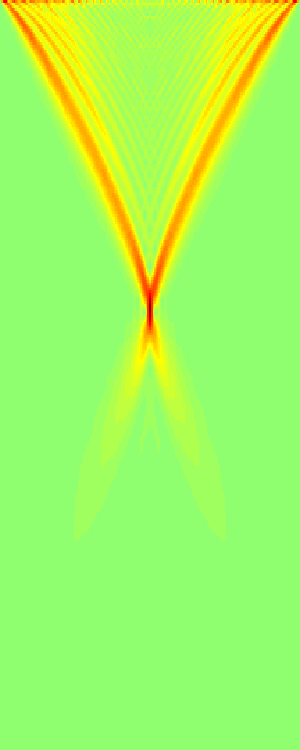
\includegraphics[height=0.5\textwidth]{assets/shear/data/F158.png}};

					% draw the borders
					\draw (0, 0) rectangle(10, 10);

					% the lesion
					\draw (6.25, 6) circle(0.5);

					% the lesion text
					\draw[<-] (6.6036, 5.6464) -- (7.25, 5);
					\draw (7.05, 5) node[right]{\scriptsize Lesion};

					% the focal point
					\draw[<-] (5, 6) -- (4, 6);
					\draw (4, 6) node[left]{\scriptsize Focal point};

					% the force distribution
					\draw[<-] (5.8, 7.75) -- (7, 7.75);
					\draw (6.8, 7.75) node[right]{\scriptsize Radiation force};

					% the focal line
					\draw[dashed] (5, 6) -- (10, 6);
					\draw[<-] (7.5, 6) -- (7.5, 6.5);
					\draw (7.5, 6.5) node[above]{\scriptsize Focal line};
				\end{tikzpicture}
				\caption[Sample radiation force distribution in relation to lesion location]{A sample acoustic radiation force distribution shown with a schematic of the lesion's location and size in the simulated tissue domain. Note how the focal point is adjacent to the lesion, offset in this case by \SI{1.25}{\cm}. The focal line extends laterally from the focal point, through the lesion, to the edge of the tissue domain---this is the line that will be used to calculate shear wave speeds.}
				\label{fig:arfi_force_shear_lesion_schematic}
			\end{figure}

		\subsection{Sample Shear Wave Speed Measurement}
		\label{subsec:shear_results_sample_wave_speed}
			Although measuring the shear wave speed of tissue may quantify the tissue stiffness through equation \ref{equ:shear_wave_speed_complex}, the results presented here represent the measured stiffness ratio of lesions in order to present continuity with Chapters \ref{chap:quasi-static} and \ref{chap:arfi}. In all cases where relative lesion stiffness is presented, it was calculated through comparison of the mean shear wave speed in the defined lesion region with the mean shear wave speed outside of the lesion region along the path of the lateral shear wave radiation direction. Specific ratios may be calculated using equation \ref{equ:shear_stiffness_ratio} where $E_{rel}$ is the relative stiffness ratio, $\mu_l$ and $\mu_t$ are Lam\'{e}'s second parameter for the lesion and tissue respectively, $c_{T,l}$ and $c_{T,t}$ are the shear wave speeds in the lesion and tissue respectively, and $\rho$ is the density of the tissue and assumed to be constant between the lesion and tissue.

			\begin{subequations}
				\label{equ:shear_stiffness_ratio}
				\begin{align}
					c_T &= \sqrt{\frac{\mu}{\rho}} \\
					c_T^2\rho &= \mu \\
					E_{rel} = \frac{\mu_l}{\mu_t} &= \left(\frac{c_{T,l}}{c_{T,t}}\right)^2
				\end{align}
			\end{subequations}

			In order to determine the velocity of generated shear waves, the ARFI load-induced displacement of the soft tissue must be tracked through time along a line passing through the focal point radiating laterally outward in the finite-element model of tissue deformation. A sample result of tissue displacement through time and along such a line is presented in Fig. \ref{fig:lateral_wave_i158} where the wave can be readily visualized through time, noting that the wave travels ever further from the centerline.

			\begin{figure}[!t]
				\centering
				\begin{tikzpicture}
					\begin{axis}[
						scale only axis,
						height=3in,
						width=\textwidth-\widthof{100}-1in,
						xlabel={Distance from centerline, $x$ (\si{\cm})},
						ylabel={Axial displacement, $v$ (\si{\um})},
						grid=major,
						legend entries={$t = \SI{2.5}{\ms}$, $t = \SI{7.5}{\ms}$, $t = \SI{12.5}{\ms}$, $t = \SI{17.5}{\ms}$, $t = \SI{22.5}{\ms}$, $t = \SI{27.5}{\ms}$},
						legend style={legend pos=south east,font=\small},
						clip=true,
						cycle list name=SmoothColourPlotCycle,
						draw=black, text=black, fill=black,
						xmin=0, xmax=5]
						\addplot table[x expr=\thisrow{x}*100, y expr=\thisrow{v}*1e6] {assets/shear/data/shear_lateral_i158_t025.dat};
						\addplot table[x expr=\thisrow{x}*100, y expr=\thisrow{v}*1e6] {assets/shear/data/shear_lateral_i158_t075.dat};
						\addplot table[x expr=\thisrow{x}*100, y expr=\thisrow{v}*1e6] {assets/shear/data/shear_lateral_i158_t125.dat};
						\addplot table[x expr=\thisrow{x}*100, y expr=\thisrow{v}*1e6] {assets/shear/data/shear_lateral_i158_t175.dat};
						\addplot table[x expr=\thisrow{x}*100, y expr=\thisrow{v}*1e6] {assets/shear/data/shear_lateral_i158_t225.dat};
						\addplot table[x expr=\thisrow{x}*100, y expr=\thisrow{v}*1e6] {assets/shear/data/shear_lateral_i158_t275.dat};
					\end{axis}
				\end{tikzpicture}
				\caption[Sample shear wave motion through time]{Axial displacement induced by a shear wave traveling laterally across the focal line of an ARFI load. There is a stiff ($E_{rel} = 3.2$) lesion with a diameter of \SI{1}{\cm} located \SI{1.25}{\cm} away from the centerline, with both the focal line and the lesion located at a depth of \SI{4}{\cm} from the surface.}
				\label{fig:lateral_wave_i158}
			\end{figure}

			The results in Fig. \ref{fig:lateral_wave_i158} represent a finite subsample of the shear wave's propagation along the focal line. For a continuous representation of the shear wave propagation, the surface shown in Fig \ref{fig:lateral_cut_i158} may be constructed. In order to track the wave through both position and time, a contour line representing a constant displacement value may be extracted. For this work, a contour line representing the mean value of the displacement over the entire position-time domain was utilized and is portrayed in Fig. \ref{fig:lateral_cut_i158_imgsc_isoline}.

			\begin{figure}[!t]
				\centering
				\begin{tikzpicture}
					\begin{axis}[
						scale only axis,
						enlargelimits=false,
						height=3in,
						width=\textwidth-\widthof{100}-1in,
						xlabel={Time, $t$ (\si{\ms})},
						ylabel={Distance from centerline, $x$ (\si{\cm})},
						axis on top,
						colormap name={RdBu},
						colorbar, point meta min=-6.6746e-01, point meta max=3.8648e-01, colorbar style={at={(1.05,0)}, anchor=south west, width=0.03\textwidth, ylabel={Axial Displacement, $v$ (\si{\um})},
							draw=black, text=black, fill=black}]
							\addplot graphics[xmin=0,xmax=31.7,ymin=0,ymax=5]{assets/shear/data/lateralCut158.png};
					\end{axis}
				\end{tikzpicture}
				\caption[Sample continuous surface plot of shear wave induced displacement]{Continous surface plot of the shear wave induced axial displacement tracked through both time and distance from the transducer centerline. The sharp transition from negative to positive displacement marks the location of shear wave in time at any given location.}
				\label{fig:lateral_cut_i158}
			\end{figure}

			\begin{figure}[!t]
				\centering
				\begin{tikzpicture}
					\begin{axis}[
						scale only axis,
						enlargelimits=false,
						height=3in,
						width=\textwidth-\widthof{100}-1in,
						xlabel={Time, $t$ (\si{\ms})},
						ylabel={Distance from centerline, $x$ (\si{\cm})},
						axis on top,
						colormap name={RdBu},
						colorbar, point meta min=-6.6746e-01, point meta max=3.8648e-01, colorbar style={at={(1.05,0)}, anchor=south west, width=0.03\textwidth, ylabel={Axial Displacement, $v$ (\si{\um})}, draw=black, text=black, fill=black}]
							\addplot graphics[xmin=0,xmax=31.7,ymin=0,ymax=5]{assets/shear/data/lateralCut158.png};
							\addplot[draw=black, solid, ultra thick] table[x expr=\thisrow{t}*1000, y expr=\thisrow{x}*100] {assets/shear/data/shear_lateral_i158_isoline.dat};
							\draw[ultra thick, <->, draw=black] (axis cs:15,0.75) -- (axis cs:15,1.75);
							\draw[ultra thick, draw=black, dashed] (axis cs:0,0.75) -- (axis cs:17.5,0.75);
							\draw[ultra thick, draw=black, dashed] (axis cs:0,1.75) -- (axis cs:17.5,1.75);
							\node[right] at (axis cs:15,1.25) {Lesion};
							\draw[ultra thick, ->, draw=black] (axis cs:25.65,2.75) -- (axis cs:25.65,3.7755102040816);
							\node[below] at (axis cs:25.65,2.75) {Iso-line};
					\end{axis}
				\end{tikzpicture}
				\caption[Sample continuous surface plot of shear wave induced axial displacement highlighting the shear wave location in time]{Continuous surface plot of shear wave induced axial displacement highlighting a mean contour line representing the shear wave location as time progresses. By inspection, the slope of the contour line is greater within the lesionous region than outside of it, suggesting that the lesion is stiffer than the surrounding tissue.}
				\label{fig:lateral_cut_i158_imgsc_isoline}
			\end{figure}

			Fig. \ref{fig:lateral_cut_i158_isoline} represents the extracted contour line. This contour line now represents a position-time trace of the shear wave, from which the velocity of the wave may be calculated by differentiating the position of the wave with respect to time as per equation \ref{equ:shear_speed_differentiation}. Care must be taken when numerically differentiating, as numerical errors are greatly amplified by differentiation. To combat this, a moving window average filter with a kernel of \SI{5}{\mm} was applied to the position-time curve before center-difference differentiation was used to result in the shear wave speed graph given in Fig. \ref{fig:lateral_cut_i158_shear_wave_speed}.

			\begin{equation}
				\label{equ:shear_speed_differentiation}
				c_T = \frac{dx}{dt}
			\end{equation}

			\begin{figure}[!t]
				\centering
				\begin{tikzpicture}
					\begin{axis}[
						scale only axis,
						height=3in,
						width=\textwidth-\widthof{100}-1in,
						xlabel={Time, $t$ (\si{\ms})},
						ylabel={Distance from centerline, $x$ (\si{\cm})},
						grid=major,
						clip=true,
						cycle list name=SmoothColourPlotCycle,
						draw=black, text=black, fill=black]
						\addplot table[x expr=\thisrow{t}*1000, y expr=\thisrow{x}*100] {assets/shear/data/shear_lateral_i158_isoline.dat};
					\end{axis}
				\end{tikzpicture}
				\caption[Sample extracted shear wave position-time trace]{The extracted shear wave position-time trace showing the location of the generated shear wave increases with time, albeit at different rates depending on the underlying tissue properties.}
				\label{fig:lateral_cut_i158_isoline}
			\end{figure}

			\begin{figure}[!t]
				\centering
				\begin{tikzpicture}
					\begin{axis}[
						scale only axis,
						height=3in,
						width=\textwidth-\widthof{100}-1in,
						xlabel={Distance from centerline, $x$ (\si{\cm})},
						ylabel={Measured Shear Wave Speed, $c_t$ (\si{\m\per\s})},
						grid=major,
						clip=true,
						cycle list name=SmoothColourPlotCycle,
						draw=black, text=black, fill=black]
						\addplot table[x expr=\thisrow{x}*100] {assets/shear/data/shear_lateral_i158_shear_wave_speed.dat};

						\draw[ultra thick, ->, draw=black] (axis cs:0.25,2) -- (axis cs:0.75,2);
						\draw[ultra thick, <-, draw=black] (axis cs:1.75,2) -- (axis cs:2.25,2);
						\node[right] at (axis cs:2.25,2) {Lesion};
						\draw[ultra thick, draw=black, dashed] (axis cs:0.75,0) -- (axis cs:0.75,2.05);
						\draw[ultra thick, draw=black, dashed] (axis cs:1.75,0) -- (axis cs:1.75,2.05);
					\end{axis}
				\end{tikzpicture}
				\caption[Sample trace of shear wave speed through the focal line]{Trace of the shear wave speed along the focal line through both lesionous and ``healthy'' tissue. The shear wave speed within the lesion is much greater than the shear wave speed through the ``healthy'' tissue, indicating that the lesion is significantly stiffer than the surrounding tissue. The shear wave speed was calculated as the numerical differentiation of the shear wave's position through time.}
				\label{fig:lateral_cut_i158_shear_wave_speed}
			\end{figure}

			As is shown in Fig. \ref{fig:lateral_cut_i158_shear_wave_speed}, the speed of the shear wave within the lesion (which was in this case 3.2 times as stiff as the surrounding tissue) is substantially greater than the shear wave speed in the regular tissue. Note that instead of an impulse response at the boundaries of the lesion as might be expected, the shear wave speed reaches a peak value roughly halfway through the lesion, indicating that the wave requires some minute amount of time to both speed up and slow down within the lesion, suggesting that the technique may have difficulty identifying small lesions as the shear wave speed will not be able to fully adjust to the lesion in the time it takes for the wave to completely pass through the lesion.

		\subsection{Lesion Detection Characterization}
			\note[KH]{Add and talk lesion size characterization here}

			One of the key parameters used in shear wave speed quantification is the distance between the focal point of the acoustic radiation force and the lesion itself. In order to adequately generate fully-formed shear waves within the lesion, the focal point of acoustic radiation force should be located adjacent to the lesion. As can be seen in Fig. \ref{fig:erel_doff_d4}, regardless of the lesion offset distance, shear wave speed quantification is able to differentiate lesions from the tissue with reasonable accuracy. Fig. \ref{fig:erel_doff_mse_d4} portrays the mean squared error between the measured and true lesion stiffness ratios with increasing lesion offset distance. As Fig. \ref{fig:erel_doff_mse_d4} shows, a lesion offset of approximately \SI{2.5}{\cm} is ideal for quantifying lesion stiffness as it produces the least amount of error between the true and measured lesion stiffness ratios.

			\begin{figure}[!t]
				\centering
				\begin{tikzpicture}
					\begin{axis}[
						scale only axis,
						height=3in,
						width=\textwidth-\widthof{100}-1in,
						xlabel={True Stiffness Ratio, $E_{rel,true}$},
						ylabel={Measured Stiffness Ratio, $E_{rel,measured}$},
						grid=major,
						legend entries={$\Delta_{off} = \SI{0.00}{\cm}$, $\Delta_{off} = \SI{1.25}{\cm}$, $\Delta_{off} = \SI{2.50}{\cm}$, $\Delta_{off} = \SI{3.75}{\cm}$},
						legend style={legend pos=south east,font=\small},
						clip=true,
						cycle list name=ColourPlotCycle,
						draw=black, text=black, fill=black]
						\addplot table {assets/shear/data/shear_doff_d4_o000.dat};
						\addplot table {assets/shear/data/shear_doff_d4_o125.dat};
						\addplot table {assets/shear/data/shear_doff_d4_o250.dat};
						\addplot table {assets/shear/data/shear_doff_d4_o375.dat};
					\end{axis}
				\end{tikzpicture}
				\caption[Numerical characterization of shear wave speed measured stiffness ratio with changing lesion offsets]{Numerical characterization of the shear wave speed measured stiffness ratios acquired with varying lesion offsets for a hard-boundaried \SI{0.5}{cm} radius lesion at a depth of \SI{4}{\cm} using an ARFI probing frequency of \SI{2}{\MHz}. The greatest error between the true and measured stiffness ratios occurred at the highest stiffness ratio of $3.2$, with the large lesion offset underestimating the stiffness ratio and the negated lesion offset overestimating the stiffness ratio.}
				\label{fig:erel_doff_d4}
			\end{figure}

			\begin{figure}[!t]
				\centering
				\begin{tikzpicture}
					\begin{axis}[
						scale only axis,
						height=3in,
						width=\textwidth-\widthof{100}-1in,
						major x tick style = transparent,
						ybar=2*\pgflinewidth,
						bar width=28pt,
						ymajorgrids=true,
						xlabel={Lesion Offset, $d_{off}$ (\si{\cm})},
						ylabel={Mean Squared Error},
						enlarge x limits=0.25,
						ymin=0,
						xtick=data,
						cycle list name=BarColourPlotCycle]
						\addplot table[x expr=\thisrow{doff}*100] {assets/shear/data/shear_doff_mse_d4.dat};
					\end{axis}
				\end{tikzpicture}
				\caption[Shear-wave speed quantified mean squared error related to lesion offset]{Mean squared error between the true and measured lesion stiffness ratios for increasing lesion offsets for a hard-boundaried \SI{0.5}{cm} radius lesion at a depth of \SI{4}{\cm} using an ARFI probing frequency of \SI{2}{\MHz}.}
				\label{fig:erel_doff_mse_d4}
			\end{figure}

			\note[KH]{Talk about depth characterization}

			\begin{figure}[!t]
				\centering
				\begin{tikzpicture}
					\begin{axis}[
						scale only axis,
						height=3in,
						width=\textwidth-\widthof{100}-1in,
						xlabel={True Stiffness Ratio, $E_{rel,true}$},
						ylabel={Measured Stiffness Ratio, $E_{rel,measured}$},
						grid=major,
						legend entries={$d = \SI{2}{\cm}$, $d = \SI{4}{\cm}$, $d = \SI{6}{\cm}$, $d = \SI{8}{\cm}$},
						legend style={legend pos=south east,font=\small},
						clip=true,
						cycle list name=ColourPlotCycle,
						draw=black, text=black, fill=black]
						\addplot table {assets/shear/data/shear_depth_o250_d2.dat};
						\addplot table {assets/shear/data/shear_depth_o250_d4.dat};
						\addplot table {assets/shear/data/shear_depth_o250_d6.dat};
						\addplot table {assets/shear/data/shear_depth_o250_d8.dat};
					\end{axis}
				\end{tikzpicture}
				\caption[Numerical characterization of shear wave speed measured stiffness ratio with changing lesion depth]{Numerical characterization of the shear wave speed measured stiffness ratios acquired with varying lesion and focal point depths for a hard-boundaried \SI{0.5}{cm} radius lesion with an offset of \SI{2.50}{\cm} using an ARFI probing frequency of \SI{2}{\MHz}.}
				\label{fig:erel_depth_o250}
			\end{figure}

			\begin{figure}[!t]
				\centering
				\begin{tikzpicture}
					\begin{axis}[
						scale only axis,
						height=3in,
						width=\textwidth-\widthof{100}-1in,
						major x tick style = transparent,
						ybar=2*\pgflinewidth,
						bar width=28pt,
						ymajorgrids=true,
						xlabel={Lesion Depth, $d$ (\si{\cm})},
						ylabel={Mean Squared Error},
						enlarge x limits=0.25,
						ymin=0,
						xtick=data,
						cycle list name=BarColourPlotCycle]
						\addplot table[x expr=\thisrow{depth}*100] {assets/shear/data/shear_depth_mse_o250.dat};
					\end{axis}
				\end{tikzpicture}
				\caption[Shear-wave speed quantified mean squared error related to lesion depth]{Mean squared error between the true and measured lesion stiffness ratios for increasing lesion depths for a hard-boundaried \SI{0.5}{cm} radius lesion with an offset of \SI{2.50}{\cm} using an ARFI probing frequency of \SI{2}{\MHz}.}
				\label{fig:erel_depth_mse_o250}
			\end{figure}

			\note[KH]{Present blurred lesion characterizations}

			\begin{figure}[!t]
				\centering
				\begin{tikzpicture}
					\begin{axis}[
						scale only axis,
						height=3in,
						width=\textwidth-\widthof{100}-1in,
						xlabel={True Stiffness Ratio, $E_{rel,true}$},
						ylabel={Measured Stiffness Ratio, $E_{rel,measured}$},
						grid=major,
						legend entries={$b_r = \SI{2.5}{\mm}$, $b_r = \SI{5.0}{\mm}$, $b_r = \SI{7.5}{\mm}$},
						legend style={legend pos=south east,font=\small},
						clip=true,
						cycle list name=ColourPlotCycle,
						draw=black, text=black, fill=black]
						\addplot table {assets/shear/data/shear_blur_r25.dat};
						\addplot table {assets/shear/data/shear_blur_r50.dat};
						\addplot table {assets/shear/data/shear_blur_r75.dat};
					\end{axis}
				\end{tikzpicture}
				\caption[Numerical characterization of shear wave speed measured stiffness ratio with blurred lesions]{Numerical characterization of the shear wave speed measured stiffness ratios acquired with varying lesion and focal point depths for a blurred \SI{1.0}{cm} radius lesion with an offset of \SI{1.25}{\cm} at a depth of \SI{4}{\cm} using an ARFI probing frequency of \SI{2}{\MHz}.}
				\label{fig:erel_blur}
			\end{figure}

			\begin{figure}[!t]
				\centering
				\begin{tikzpicture}
					\begin{axis}[
						scale only axis,
						height=3in,
						width=\textwidth-\widthof{100}-1in,
						major x tick style = transparent,
						ybar=2*\pgflinewidth,
						bar width=28pt,
						ymajorgrids=true,
						xlabel={Lesion Blur Radius, $b_r$ (\si{\mm})},
						ylabel={Mean Squared Error},
						enlarge x limits=0.25,
						ymin=0,
						xtick=data,
						cycle list name=BarColourPlotCycle]
						\addplot table[x expr=\thisrow{blur}*1000] {assets/shear/data/shear_blur_mse.dat};
					\end{axis}
				\end{tikzpicture}
				\caption[Shear-wave speed quantified mean squared error related to lesion blurring]{Mean squared error between the true and measured lesion stiffness ratios for increasing lesion depths for a blurred \SI{1.0}{cm} radius lesion with an offset of \SI{1.25}{\cm} at a depth of \SI{4}{\cm} using an ARFI probing frequency of \SI{2}{\MHz}.}
				\label{fig:erel_blur_mse}
			\end{figure}

			\note[KH]{Present clustered lesion density characterizations}

			\begin{figure}[!t]
				\centering
				\begin{tikzpicture}
					\begin{axis}[
						scale only axis,
						height=3in,
						width=\textwidth-\widthof{100}-1in,
						xlabel={True Stiffness Ratio, $E_{rel,true}$},
						ylabel={Measured Stiffness Ratio, $E_{rel,measured}$},
						grid=major,
						legend entries={$b_\rho = \SI{10}{\per\cm\squared}$, $b_\rho = \SI{20}{\per\cm\squared}$, $b_\rho = \SI{30}{\per\cm\squared}$, $b_\rho = \SI{40}{\per\cm\squared}$},
						legend style={legend pos=south east,font=\small},
						clip=true,
						cycle list name=ColourPlotCycle,
						draw=black, text=black, fill=black]
						\addplot table {assets/shear/data/shear_cluster_dens_d10.dat};
						\addplot table {assets/shear/data/shear_cluster_dens_d20.dat};
						\addplot table {assets/shear/data/shear_cluster_dens_d30.dat};
						\addplot table {assets/shear/data/shear_cluster_dens_d40.dat};
					\end{axis}
				\end{tikzpicture}
				\caption[Numerical characterization of shear wave speed measured stiffness ratio with clustered lesions]{Numerical characterization of the shear wave speed measured stiffness ratios acquired with varying cluster densities for clustered \SI{1}{\mm} radius lesions within a \SI{1.0}{cm} radius with an offset of \SI{1.25}{\cm} at a depth of \SI{4}{\cm} using an ARFI probing frequency of \SI{2}{\MHz}.}
				\label{fig:erel_cluster_density}
			\end{figure}

			\begin{figure}[!t]
				\centering
				\begin{tikzpicture}
					\begin{axis}[
						scale only axis,
						height=3in,
						width=\textwidth-\widthof{100}-1in,
						major x tick style = transparent,
						ybar=2*\pgflinewidth,
						bar width=28pt,
						ymajorgrids=true,
						xlabel={Lesion Cluster Density, $b_\rho$ (\si{\per\cm\squared})},
						ylabel={Mean Squared Error},
						enlarge x limits=0.25,
						ymin=0,
						xtick=data,
						cycle list name=BarColourPlotCycle]
						\addplot table {assets/shear/data/shear_cluster_dens_mse.dat};
					\end{axis}
				\end{tikzpicture}
				\caption[Shear-wave speed quantified mean squared error related to small lesion cluster density]{Mean squared error between the true and measured lesion stiffness ratios for increasing lesion cluster density for clustered \SI{1}{\mm} radius lesions within a \SI{1.0}{cm} radius with an offset of \SI{1.25}{\cm} at a depth of \SI{4}{\cm} using an ARFI probing frequency of \SI{2}{\MHz}.}
				\label{fig:erel_cluster_density_mse}
			\end{figure}

			\note[KH]{Present clustered lesion radius characterizations}

			\begin{figure}[!t]
				\centering
				\begin{tikzpicture}
					\begin{axis}[
						scale only axis,
						height=3in,
						width=\textwidth-\widthof{100}-1in,
						xlabel={True Stiffness Ratio, $E_{rel,true}$},
						ylabel={Measured Stiffness Ratio, $E_{rel,measured}$},
						grid=major,
						legend entries={$r_{bl} = \SI{0.5}{\mm}$, $r_{bl} = \SI{1.0}{\mm}$, $r_{bl} = \SI{1.5}{\mm}$},
						legend style={legend pos=south east,font=\small},
						clip=true,
						cycle list name=ColourPlotCycle,
						draw=black, text=black, fill=black]
						\addplot table {assets/shear/data/shear_cluster_radius_r05.dat};
						\addplot table {assets/shear/data/shear_cluster_radius_r10.dat};
						\addplot table {assets/shear/data/shear_cluster_radius_r15.dat};
					\end{axis}
				\end{tikzpicture}
				\caption[Numerical characterization of shear wave speed measured stiffness ratio with clustered lesions]{Numerical characterization of the shear wave speed measured stiffness ratios acquired with varying clustered lesion radii for clustered lesions with a density of \SI{30}{\per\cm\squared} within a \SI{1.0}{cm} radius with an offset of \SI{1.25}{\cm} at a depth of \SI{4}{\cm} using an ARFI probing frequency of \SI{2}{\MHz}.}
				\label{fig:erel_cluster_radius}
			\end{figure}

			\begin{figure}[!t]
				\centering
				\begin{tikzpicture}
					\begin{axis}[
						scale only axis,
						height=3in,
						width=\textwidth-\widthof{100}-1in,
						major x tick style = transparent,
						ybar=2*\pgflinewidth,
						bar width=28pt,
						ymajorgrids=true,
						xlabel={Clustered Lesion Radius, $r_{bl}$ (\si{\mm})},
						ylabel={Mean Squared Error},
						enlarge x limits=0.25,
						ymin=0,
						xtick=data,
						cycle list name=BarColourPlotCycle]
						\addplot table {assets/shear/data/shear_cluster_radius_mse.dat};
					\end{axis}
				\end{tikzpicture}
				\caption[Shear-wave speed quantified mean squared error related to small lesion cluster density]{Mean squared error between the true and measured lesion stiffness ratios for increasing clustered lesion radii for clustered lesions with a density of \SI{30}{\per\cm\squared} within a \SI{1.0}{cm} radius with an offset of \SI{1.25}{\cm} at a depth of \SI{4}{\cm} using an ARFI probing frequency of \SI{2}{\MHz}.}
				\label{fig:erel_cluster_radius_mse}
			\end{figure}

			\note[KH]{Present visible human lesion characterizations}

		\subsection{Physical Phantom Validation}
			\note[KH]{Present physical phantom validation}

	\section{Conclusions}
		